\section{Fundamentos de bases de datos}

En esta sección, veremos de forma introductoria esos fundamentos de bases de datos genéricas, aplicables a cualquier ámbito \cite{ref2}.

\subsection*{¿Qué es una base de datos?}

Entendemos como \texttt{Base de Datos} un conjunto de datos estructurado y almacenado de forma sistemática con objeto de facilitar su posterior utilización. Una base de datos puede, por tanto, constituirse con cualquier tipo de datos.

\subsection*{¿Por qué interesa usar una base de datos?}

Las ventajas de utilizar un almacenamiento estructurado se aprecian en diversos puntos, ya que afectan no solo a los datos sino también al propio uso que se hace de estos. Algunas ventajas que afectan directamente a los datos son las siguientes \cite{ref3}:

\begin{itemize}
   \item \textbf{Mayor independencia.} Los datos son independientes de las aplicaciones que los usan, así como de los usuarios.
   
    \item \textbf{Mayor disponibilidad.} Se facilita el acceso a los datos desde contextos, aplicaciones y medios distintos, haciéndolos útiles para un mayor número de usuarios.
    
    \item \textbf{Mayor seguridad (protección de los datos).} Por ejemplo, resulta más fácil replicar una base de datos para mantener una copia de seguridad que hacerlo con un conjunto de ficheros almacenados de forma no estructurada. Además, al estar centralizado el acceso a los datos, existe una verdadera sincronización de todo el trabajo que se haya podido hacer sobre estos (modificaciones), con lo que esa copia de seguridad servirá a todos los usuarios.
    
    \item \textbf{Menor redundancia.} Un mismo dato no se encuentra almacenado en múltiples ficheros o con múltiples esquemas distintos, sino en una única instancia en la base de datos. Esto redunda en menor volumen de datos y mayor rapidez de acceso.
    
    \item \textbf{Mayor eficiencia en la captura, codificación y entrada de datos.} 
\end{itemize}

Esto tiene una consecuencia directa sobre los resultados que se obtienen de la explotación de la base de datos, presentándose al respecto ventajas como, por ejemplo:

\begin{itemize}
 \item \textbf{Mayor coherencia.} La mayor calidad de los datos que se deriva de su mejor gestión deriva en mayor calidad de los resultados.
 
 \item \textbf{Mayor eficiencia.} Facilitando el acceso a los datos y haciendo más sencilla su explotación, la obtención de resultados es más eficiente.
 
 \item \textbf{Mayor valor informativo.} Resulta más sencillo extraer la información que los datos contienen, ya que uno de los cometidos de la base de datos es aumentar el valor de estos como fuente de información. 
\end{itemize}

De forma resumida, puede decirse que la principal bondad de una base de datos es la centralización que supone de todos los datos con los que se trabaja en un contexto determinado, con las consecuencias que ello tiene para una mejor gestión, acceso o estructuración de estos.

\subsection*{Tipos de base de datos}

Existen varios tipos de bases de datos; cada tipo de base de datos tiene su propio modelo de datos (la manera de cómo están estructurados). Entre ellas se incluyen \cite{ref4}:

\subsubsection*{Modelo de base de datos plana}

En un modelo de base de datos plano, hay dos dimensiones (estructura plana) de conjunto de datos. Hay una columna de información y dentro de esta columna, se supone que cada dato tendrá que ver con la columna.

Por ejemplo, un modelo de base de datos plana que sólo incluye códigos postales. Dentro de la base de datos, sólo habrá una columna y cada nueva fila dentro de una columna será un nuevo código postal.

\begin{figure}[!h]
	\centering
	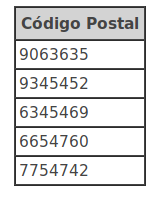
\includegraphics[scale=0.5]{images/tipo_plana}
	\caption{Ejemplo de base de datos plana}
	\label{fig:bd_plana}
\end{figure}

\subsubsection*{Modelo de base de datos jeŕarquica}

El modelo jerárquico de bases de datos se asemeja a la estructura de un árbol, tal como Microsoft Windows organiza las carpetas y archivos. En un modelo jerárquico de bases de datos, cada enlace es anidado con el fin de conservar los datos organizados en un orden particular en un mismo nivel de lista. Por ejemplo, una base de datos jerárquico de ventas, puede incluir las ventas de cada día como un archivo separado. Anidadas dentro de este archivo están todas las ventas (el mismo tipo de datos) para el día.

\begin{figure}[!h]
	\centering
	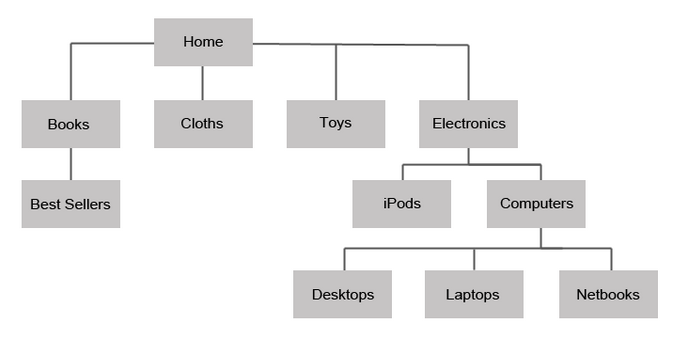
\includegraphics[scale=0.5]{images/tipo_jerarquica}
	\caption{Ejemplo de base de datos jerárquica}
	\label{fig:bd_jerarquica}
\end{figure}

\subsubsection*{Modelo de red}

En un modelo de red, la característica definitoria es que se almacena un registro con un enlace a otros registros - en efecto,una red.

Estas redes (o, a veces, a que se refiere como punteros) puede ser una variedad de diferentes tipos de información como números de nodo de un disco o incluso la dirección. 

\begin{figure}[!h]
	\centering
	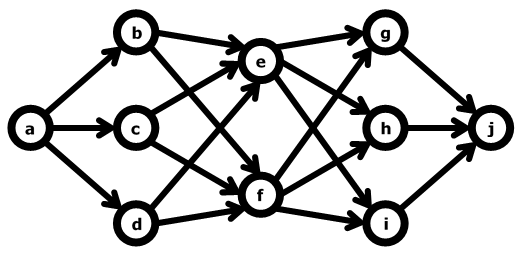
\includegraphics[scale=0.55]{images/tipo_red}
	\caption{Ejemplo de base de datos en red}
	\label{fig:bd_red}
\end{figure}

\subsubsection*{Modelo de bases de datos relacionales}

Las  bases  de  datos  relacionales son un  tipo  de  base  de  datos  que  cumple  con  el  modelo relacional.Consisten en bases de datos separadas en tablas donde cada columna representa un campo y cada fila representa un registro.Cada fila de la tabla tiene una clave única.Las tablas se pueden vincular entre sí con el uso de claves externas o columnas comunes.

\begin{figure}[!h]
	\centering
	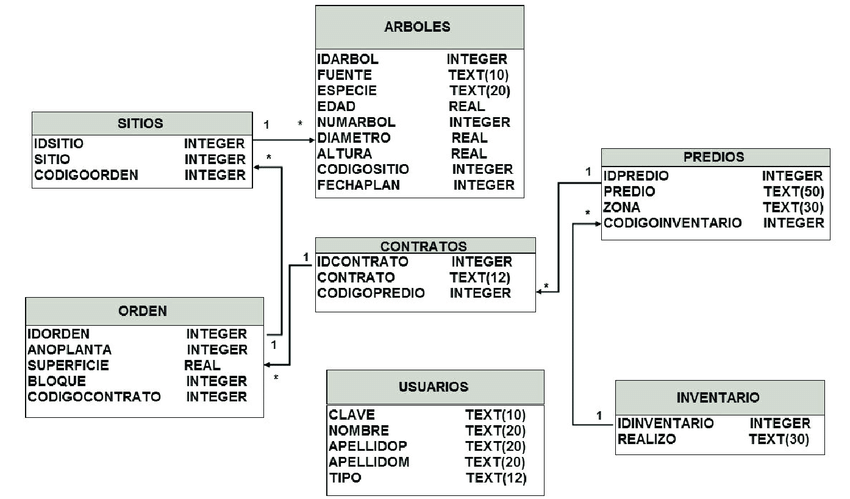
\includegraphics[scale=0.5]{images/tipo_relacional}
	\caption{Ejemplo de base de datos relacional}
	\label{fig:bd_relacional}
\end{figure}

\subsubsection*{Modelo de bases de datos NoSQL}

El término NoSQL que significa Not only SQL(No solamente SQL) fue utilizado por primera vez en 1998 por Carlo Strozzipara nombrar su base de datos de fuente abierta Strozzi NoSQL que no seguía el estándar SQL, pero seguía siendo relacional.

No fue hasta el 2009 cuando Johan Oskarsson, reintrodujo el término NoSQL con la finalidad de etiquetar la aparición de sistemas de almacenamiento de datos distribuidos no relacionales.Una base de datos NoSQL proporciona un mecanismo para el almacenamiento y recuperación de los datos en medios distintos a los utilizados en las bases de datos relacionales.

\begin{figure}[!h]
	\centering
	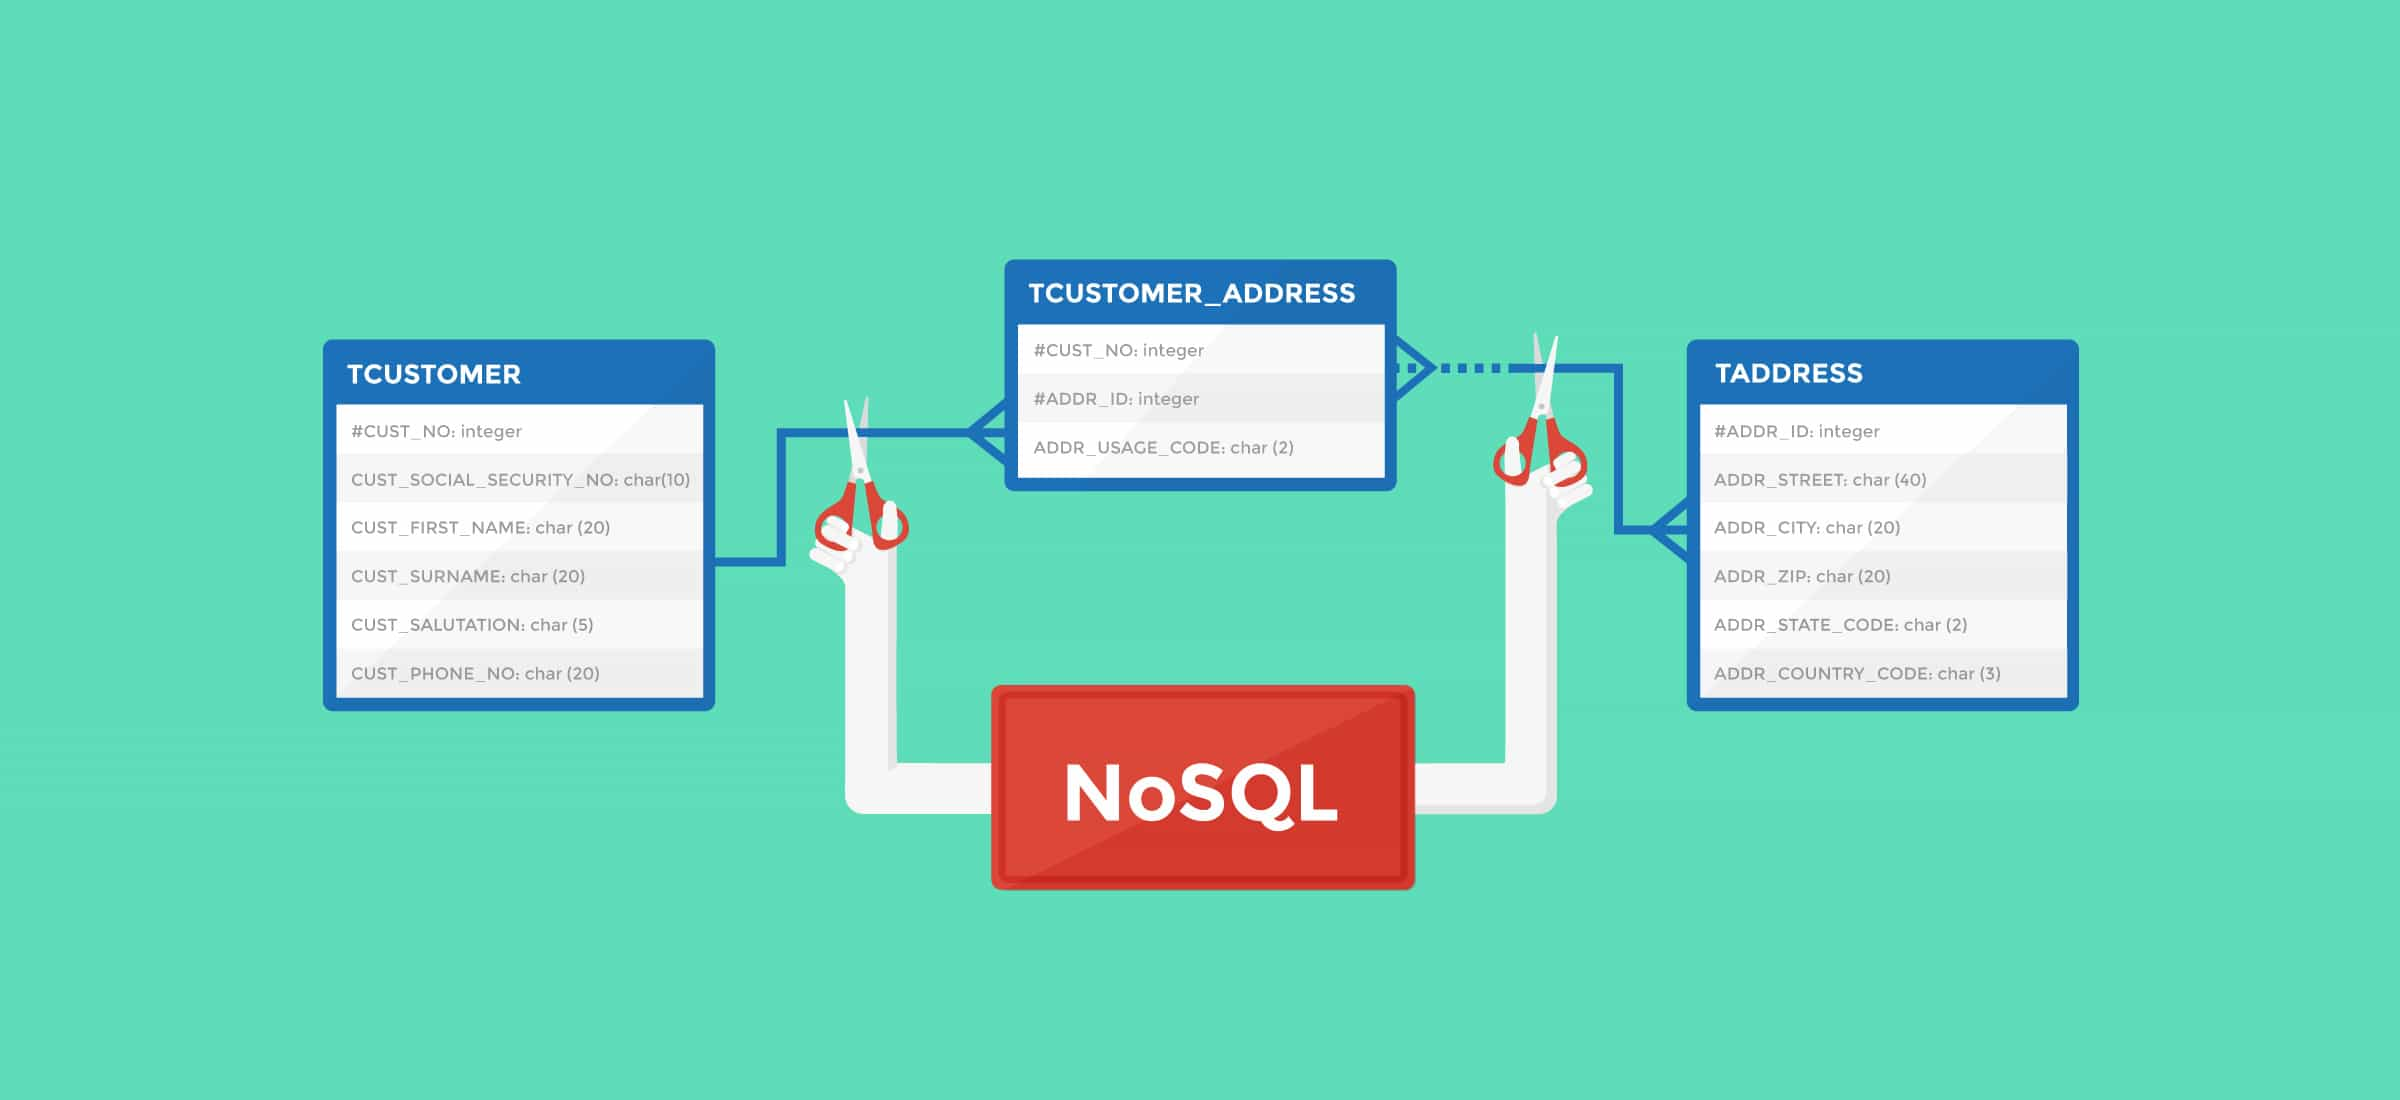
\includegraphics[scale=0.09]{images/tipo_nosql}
	\label{fig:bd_nosql}
\end{figure}

\newpage

\subsection*{Sistema gestor de base de datos}

Un \texttt{sistema gestor de bases de datos} (SGBD) es una aplicación que permite a los usuarios definir, crear y mantener una base de datos, y proporciona acceso controlado a la misma \cite{ref5}.

En general, un SGBD proporciona los siguientes servicios:

\begin{itemize}
	\item Permite la \textbf{definición de la base de datos} mediante el lenguaje de definición de datos (DDL – Data Description Language). Este lenguaje permite especificar la estructura y el tipo de los datos, así como las restricciones sobre los datos. Todo esto se almacenará en la base de datos.
	
	\item Permite la \textbf{inserción, actualización, eliminación y consulta de datos} mediante el lenguaje de manejo o manipulación de datos (DML - Data Manipulation Language). Proporciona un acceso controlado a la base de datos mediante:
	\begin{itemize}
        \item Un sistema de \textbf{seguridad}, de modo que los usuarios no autorizados no puedan acceder a la base de datos, mediante el lenguaje de control de datos (DCL - Data Control Language).
        
        \item Un sistema de \textbf{integridad} que mantiene la integridad y la consistencia de los datos.
        
        \item Un sistema de control de \textbf{concurrencia} que permite el acceso compartido a la base de datos.
        
        \item Un sistema de control de \textbf{recuperación} que restablece la base de datos después de que se produzca un fallo del hardware o del software.
        
        \item Un \textbf{diccionario de datos o catálogo} accesible por el usuario que contiene la descripción de los datos de la base de datos.
	\end{itemize}
\end{itemize}

\newpage